\documentclass[10pt,a4paper,hidelinks]{article}
\usepackage[utf8]{inputenc}
\usepackage[english]{babel}
\usepackage[T1]{fontenc}

\newcommand{\documentStatus}{DRAFT}


\usepackage{amsmath}
\usepackage{amsfonts}
\usepackage{amssymb}
\usepackage{graphicx}
\usepackage{lmodern}
\usepackage{tikz}
\usetikzlibrary{positioning}
\usetikzlibrary{shapes,snakes}
\usepackage{epigraph} 
\usepackage[left=2.5cm,
            right=2.5cm,
            top=2cm,
            bottom=2cm]{geometry}
\usepackage{setspace}
\usepackage{caption}
\usepackage{subcaption}
\usepackage{epigraph}
\usepackage{pdflscape}
\usepackage{pgfplots}

\usepackage{titlesec}
\usepackage{tcolorbox}
\usepackage{background}
\usepackage{url}
\usepackage[pdfauthor={Pierre Jézégou},
            pdftitle={ADS assignement},
            pdfsubject={Word games},
            pdfkeywords={}]{hyperref}
\usepackage{wrapfig}

\backgroundsetup{contents=\documentStatus, color=\watermarkColor}

\usepackage{fancyhdr}
\usepackage{textpos}
\usepackage{sectsty}
\usepackage{xcolor}

\setlength{\parindent}{0pt}

%%%%%%%%%%%%%%% Colors %%%%%%%%%%%%%%%
\subsectionfont{\color{fib_red}}
\subsubsectionfont{\color{fib_red}}
\renewcommand\fbox{\fcolorbox{black}{fib_red!20}}

\definecolor{fib_red}{RGB}{191,21,64}
\definecolor{fib_gray}{RGB}{111,111,111}
\definecolor{blue_upc}{RGB}{52,120,186}

\usepackage{listings}
\lstdefinestyle{mystyle}{
  backgroundcolor=\color{gray!10},
  stringstyle=\color{green!50!black},
  keywordstyle=\color{fib_red},
  numberstyle=\tiny\color{fib_gray},
  commentstyle=\color{blue_upc},
  basicstyle=\ttfamily\footnotesize,
  breakatwhitespace=false,         
  breaklines=true,                 
  captionpos=b,                    
  keepspaces=true,                 
  numbers=left,                    
  numbersep=5pt,                  
  showspaces=false,                
  showstringspaces=false,
  showtabs=false,                  
  tabsize=2
}

\lstset{style=mystyle}

\usepackage[Bjornstrup]{fncychap}
\newcommand{\watermarkColor}{red!10}


\onehalfspacing


\newcommand\VRule[1][\arrayrulewidth]{\vrule width #1}
\usepackage{xcolor,colortbl}

\newtcolorbox{mybox}[1]{
    arc=5pt,
    boxrule=0pt,
    colback=#1,
    width=\linewidth,
    halign=left,
}

\newenvironment{framed}[3]{
    \vspace*{0.5em}
    \begin{mybox}{#3!10}
        \textbf{#1}:\hfill \textit{#2}\\
        \hrule\vspace*{1em}
}
{\end{mybox}}

\newenvironment{exercise_description}[1]{
    \begin{framed}{Exercise description}{#1}{orange}
}
{\end{framed}}

\newenvironment{summary}{
    \begin{framed}{Summary}{Section \thesection}{blue}
}
{\end{framed}}


\newcommand{\colorverb}[2]{\textcolor{#1}{\texttt{\detokenize{#2}}}}
\newcommand{\type}[1]{\colorverb{green!50!black}{#1}}
\newcommand{\code}[1]{\colorverb{green!50!black}{#1}}


\usepackage{lmodern}
\renewcommand*\familydefault{\sfdefault}


\fancyfoot[R]{\raisebox{-0.5\baselineskip}{
\includegraphics[scale=0.25]{images/logos/upc_logo.jpeg}}}

\begin{document}
\pagestyle{plain}
\backgroundsetup{contents=,color=red!30}
\pagecolor{white}

\begin{center}
    \color{red!50!white}
    \textbf{\huge{STATUT - \documentStatus}}
\end{center}

\vfill


\color{black}
\begin{center}
    
\includegraphics[height=2cm]{images/logos/upc_logo.jpeg} \\
    % \vfill
    % 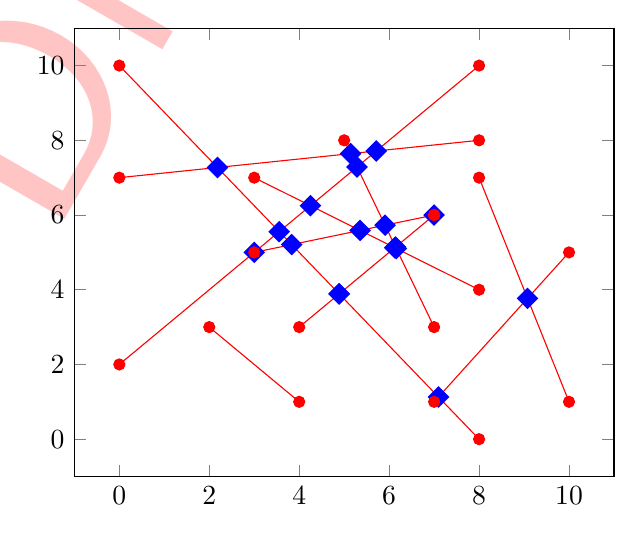
\begin{tikzpicture}
    \begin{axis}
        % Segments
        
            \addplot[red, mark=*] coordinates {(4, 3) (7, 6)};
        
            \addplot[red, mark=*] coordinates {(3, 5) (7, 6)};
        
            \addplot[red, mark=*] coordinates {(5, 8) (7, 3)};
        
            \addplot[red, mark=*] coordinates {(7, 1) (10, 5)};
        
            \addplot[red, mark=*] coordinates {(0, 7) (8, 8)};
        
            \addplot[red, mark=*] coordinates {(8, 7) (10, 1)};
        
            \addplot[red, mark=*] coordinates {(0, 2) (8, 10)};
        
            \addplot[red, mark=*] coordinates {(2, 3) (4, 1)};
        
            \addplot[red, mark=*] coordinates {(3, 7) (8, 4)};
        
            \addplot[red, mark=*] coordinates {(0, 10) (8, 0)};
        
        % Intersections
        
            \node[diamond,fill=blue, inner sep=2pt] at (axis cs:3.5555555555555554, 5.555555555555555) {};
        
            \node[diamond,fill=blue, inner sep=2pt] at (axis cs:4.888888888888889, 3.8888888888888884) {};
        
            \node[diamond,fill=blue, inner sep=2pt] at (axis cs:6.157894736842105, 5.105263157894737) {};
        
            \node[diamond,fill=blue, inner sep=2pt] at (axis cs:4.25, 6.25) {};
        
            \node[diamond,fill=blue, inner sep=2pt] at (axis cs:2.1818181818181817, 7.272727272727273) {};
        
            \node[diamond,fill=blue, inner sep=2pt] at (axis cs:4.888888888888889, 3.888888888888889) {};
        
            \node[diamond,fill=blue, inner sep=2pt] at (axis cs:7.096774193548387, 1.129032258064516) {};
        
            \node[diamond,fill=blue, inner sep=2pt] at (axis cs:3.8333333333333335, 5.208333333333333) {};
        
            \node[diamond,fill=blue, inner sep=2pt] at (axis cs:5.142857142857143, 7.642857142857143) {};
        
            \node[diamond,fill=blue, inner sep=2pt] at (axis cs:5.714285714285714, 7.714285714285714) {};
        
            \node[diamond,fill=blue, inner sep=2pt] at (axis cs:6.142857142857142, 5.142857142857143) {};
        
            \node[diamond,fill=blue, inner sep=2pt] at (axis cs:7.0, 6.0) {};
        
            \node[diamond,fill=blue, inner sep=2pt] at (axis cs:6.125, 5.125) {};
        
            \node[diamond,fill=blue, inner sep=2pt] at (axis cs:5.909090909090909, 5.7272727272727275) {};
        
            \node[diamond,fill=blue, inner sep=2pt] at (axis cs:5.285714285714286, 7.285714285714286) {};
        
            \node[diamond,fill=blue, inner sep=2pt] at (axis cs:9.076923076923077, 3.769230769230769) {};
        
            \node[diamond,fill=blue, inner sep=2pt] at (axis cs:5.352941176470589, 5.588235294117647) {};
        
            \node[diamond,fill=blue, inner sep=2pt] at (axis cs:3.0, 5.0) {};
        
    \end{axis}
\end{tikzpicture}

    \vfill
    \rule{\linewidth}{0.5mm} \\[1cm]
    {\Huge \textsc{\textcolor{fib_red}{Implementation of Sweep Lines}}}\\[1cm]
    {\Large \textsc{Assignment}}\\[0.4cm]
    {\huge \textsc{\textbf{Advanced data structures}}}\\[1cm]
    {\Large \textsc{Master in Research and Innovation - UPC}}\\[0.4cm]
    \rule{\linewidth}{0.5mm} \\[1.5cm]
\end{center}

\vfill

\textbf{Author:}
\begin{itemize}
\item Pierre \textsc{Jézégou}\newline
\textit{(Engineering student at École Centrale de Lille, Exchange student at UPC)}
\end{itemize}

\newpage
\color{black}
\pagecolor{white}
\pagestyle{fancy}
\tableofcontents

\section{Introduction}
\subsection{Sweep lines}
The Segment Intersection Problem is a classic problem in computational geometry. It involves finding all the intersections between a set of line segments in the plane. This problem has various applications, such as in computer graphics, robotics, and geographic information systems.\\

There are several algorithms to solve the Segment Intersection Problem, and one popular approach is the Sweep Line Algorithm. This algorithm involves sweeping a vertical line across the plane and processing the line segments as they are encountered by the sweep line.
To implement the Sweep Line Algorithm, we need to define the data structures and events that will be used. The data structures typically include a status structure to store the line segments that intersect the current sweep line position, and a priority queue to handle the events.\\
The events in the Sweep Line Algorithm correspond to the endpoints of the line segments. As the sweep line encounters an endpoint, it triggers an event that updates the status structure and performs any necessary computations.\\

By implementing the Sweep Line Algorithm, we can efficiently find all the intersections between the line segments and solve the Segment Intersection Problem.


\subsection{Project information}
All the source code (programs, documentation and image generators) is available in the GitHub respository dedicated to the project: https://github.com/pierre-jezegou/sweep-lines

For performance testing of algorithms, we use a MacBook Air with the M2 processor. This hardware provides ample computing power to execute our algorithms efficiently, ensuring swift analysis of their performance. As recommended, this report has been written in \LaTeX.


\section{Sweep Line Algorithm implementation}
\subsection{Structures}
\subsubsection{Point}

\subsubsection{Segment}
\paragraph{Intersection of 2 segments}
The intersection of two line segments can be determined using the concept of linear algebra, specifically by analyzing the determinant of a matrix formed by pairs of points. Given two line segments defined by points $P_1(x_1, y_1)$ and $P_2(x_2, y_2)$ for the first segment, and $Q_1(x_3, y_3)$ and $Q_2(x_4, y_4)$ for the second segment, we form two vectors representing each line segment: vector $P$ from $P_1$ to $P_2$ and vector $Q$ from $Q_1$ to $Q_2$.\\
$$P = \begin{pmatrix}
x_2 - x_1\\
y_2 - y_1
\end{pmatrix}\qquad
Q = \begin{pmatrix}
x_4 - x_3\\
y_4 - y_3
\end{pmatrix}$$

$$M = \begin{pmatrix}
x_2 - x_1 & x_4 - x_3\\
y_2 - y_1 & y_4 - y_3
\end{pmatrix}$$

The intersection of the two line segments occurs if and only if the determinant of the matrix $M$ formed by vectors $P$ and $Q$ is non-zero. Geometrically, this determinant represents the area formed by the parallelogram spanned by the two vectors. If the determinant is non-zero, it indicates that the two vectors are not collinear, meaning the two line segments intersect. Conversely, if the determinant is zero, it implies that the two vectors are collinear, and the line segments do not intersect.\\
As a consequence, the determinant of the matrix $M$ can be used to determine the intersection of two line segments. The determinant is calculated as follows:
$$\mathrm{det}(M) = (x_2 - x_1)(y_4 - y_3) - (y_2 - y_1)(x_4 - x_3)$$

Be careful, this formula only gives the intersection point of the two lines, not the intersection point of the two segments. To determine the intersection point of the two segments, we must verify that the intersection point lies within the bounds of both segments. This can be done by checking that the intersection point lies within the bounding box of both segments. If the intersection point satisfies this condition, it is the intersection point of the two segments. Otherwise, the two segments do not intersect.\\
The bounding box of a line segment is defined by the minimum and maximum x and y coordinates of the two endpoints of the segment. The intersection point of the two segments is within the bounding box of both segments if its x and y coordinates lie within the bounding boxes of both segments.\\

Let $I=(x_i, y_i)$ the potential int point. $I$ is the intersection point of the two segments if and only if $I$ is in the bounding box of both segments.
$$x_i \in [x_{min}, x_{max}], y_i \in [y_{min}, y_{max}]\qquad \text{with}
\left\lbrace\begin{array}{l}
x_{min} = \min_{i\in[1, 4]}\{x_i\}\\
x_{max} = \max_{i\in[1, 4]}\{x_i\}\\
y_{min} = \min_{i\in[1, 4]}\{y_i\}\\
y_{max} = \max_{i\in[1, 4]}\{y_i\}
\end{array}\right.$$

\subsection{Event driven}
\subsection{Structures used}

\section{Tests and results}
\subsection{Examples implementation}
\subsubsection{First example}
\subsubsection{Second example}
\subsection{Performance tests}
\subsection{Results}

\section{Conclusions}
\section{Appendix}
\lstinputlisting[firstline=1,lastline=50, language=Python]{../additional_algorithms/graphic_sweep_lines.py}

\newpage
\listoffigures
\lstlistoflistings
\listoftables

\input{../random_segments_2.tex}
\input{../tikz.tex}

\end{document}
